\vspace{-0.25em}
\section{Gdev Ecosystem}
\label{sec:ecosystem}
\vspace{-0.25em}

\begin{figure}[t]
 \begin{center}
  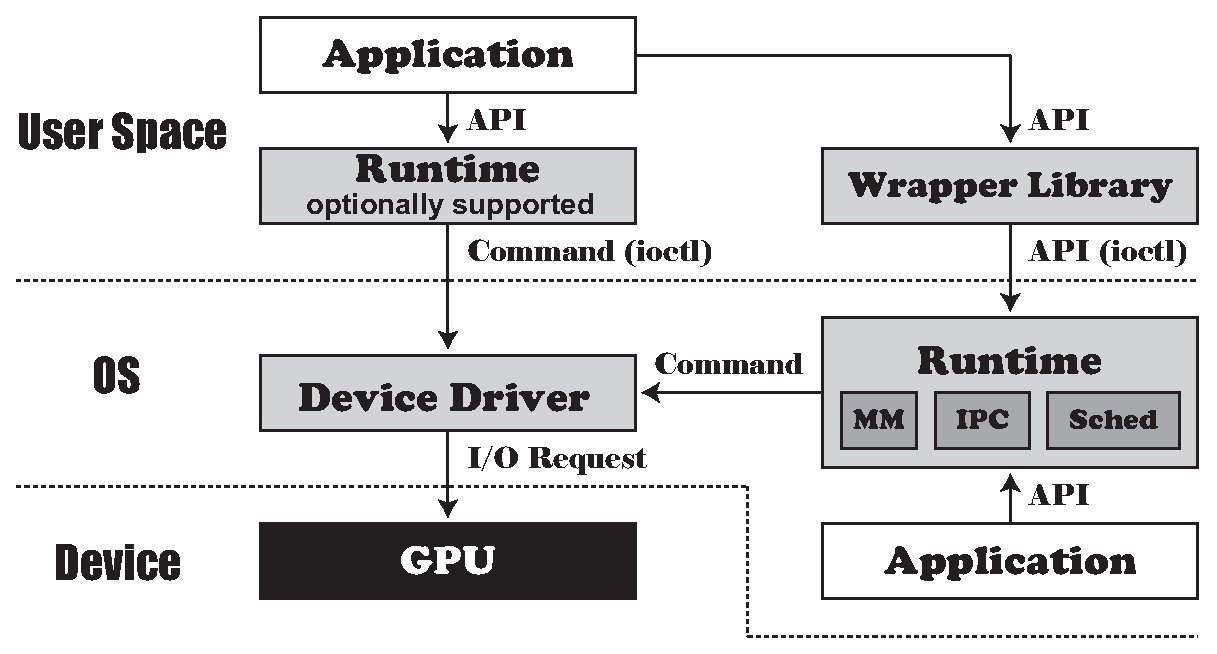
\includegraphics[width=0.863\hsize]{eps/gdev.eps}\\
  \vspace{-0.5em}
  \caption{Logical view of Gdev ecosystem.}
  \label{fig:gdev}
 \end{center}
 \vspace{-1.5em}
\end{figure}

Gdev is aimed at extending GPU resource management capabilities and a
class of applications that can benefit from the GPU.
To this end, it integrates runtime support into the OS.
Figure~\ref{fig:gdev} illustrates the overview of the Gdev ecosystem.
First, Gdev optionally supports a traditional execution model for
compatibility\footnote{For practice use, we can disable this user-space
runtime.}, where
applications make API calls to the user-space runtime library, and the
library sends GPU commands to the device driver via the system call.
As demonstrated in previous work~\cite{Kato_ATC11}, however, it is hard
to analyze at runtime the sequence of GPU commands (there could be
hundreds of commands for one operation), and it would not be appropriate
to use resource management primitives along with command calls.
This argument motivates our Gdev approach.

Unlike traditional approaches, Gdev employs runtime support in
the OS, providing GPU resource management primitives along with API calls.
OS applications can use this runtime directly, while user-space
applications can also use it through the wrapper library provided by
Gdev, which simply relays API calls to the OS runtime using the system
call.
This runtime-unified approach enables Gdev to be API-driven, where the
scheduler, for instance, is invoked for GPU computations and host-device
data transmissions upon corresponding API calls.

\textbf{Low-Level API:}
Gdev provides a set of low-level API functions for GPU programming, as
listed in Table~\ref{tab:gdev_api}.
Programmers may use either this low-level API or a high-level API,
\textit{e.g.}, CUDA, built on top of Gdev API.
Gdev supports several other API functions, including asynchronous data
transmission, but they are not within the scope of this paper.
Table~\ref{tab:gdev_api} presents an initial set of Gdev API.
We plan to extend it to make more functions available, such as texture
and 3-D processing.

\textbf{CUDA Support:}
In addition to Gdev API, we support CUDA Driver API~\cite{CUDA40} so
that legacy CUDA programs can perform on top of Gdev in both the user
space and OS.
The supported API functions are limited to those that can be implemented 
by the current version of Gdev API, but many legacy CUDA programs can
execute with this limited set of API, as we will show in
Section~\ref{sec:evaluation}.

Gdev assumes that programs are compiled by NVIDIA CUDA Compiler
(NVCC)~\cite{CUDA40}.
Since CUDA Driver API disjoints device binary and host binary, Gdev only
needs to parse the device binary to acquire static information, such
as the code size, stack size, shared memory size, local memory size, and
parameters size, when it is loaded by the host binary.
Global memory is also dynamically allocated by the host binary at
runtime.
It should be noted that CUDA also provides a different type of API,
called Runtime API, which is more high-level than Driver API.
Our prototype implementation does not support CUDA Runtime API by
itself, but we could leverage Ocelot~\cite{Diamos_PACT10} that
translates Runtime API to Driver API, in order to run CUDA programs
written in Runtime API.

\textbf{First-Class Resource Management:}
Gdev provides first-class memory management and scheduling for the GPU
to allow time-sharing multi-tasking systems to use the GPU efficiently,
including shared memory for IPC, swapping for large memory demands,
resource-based queuing for high-throughput, and resource partitioning
for virtual GPUs.
Our resource management scheme is also not limited to GPUs, but can be
generalized for a broad class of heterogeneous compute devices.

\begin{table}[t]
 \caption{Representatives of Gdev API.}
 \vspace{-0.5em}
 \label{tab:gdev_api}
 \begin{center}
  {\footnotesize
  \begin{tabular}{|l|l|}
   \hline
   \textbf{API name} & \textbf{Description}\\
   \hline
   \texttt{gopen}/\texttt{gclose} & Open/close the device\\
   \hline
   \texttt{gmalloc}/\texttt{gfree} & Allocate/free device memory\\
   \hline
   \texttt{gmalloc\_io}/\texttt{gfree\_io} & Allocate/free host I/O memory\\
   \hline
   \texttt{gmemcpy\_to\_device} & Copy memory to the device\\
   \hline
   \texttt{gmemcpy\_from\_device} & Copy memory from the device\\
   \hline
   \texttt{gmemcpy\_in\_device} & Copy memory within the device\\
   \hline
   \texttt{glaunch}/\texttt{gsync} & Launch/wait computation\\
   \hline
   \texttt{gquery} & Query device information\\
   \hline
   \texttt{gshmget}/\texttt{gshmctl} & Manage shared device memory\\
   \hline
   \texttt{gshmat}/\texttt{gshmdt} & Share/unshare device memory\\
   \hline
  \end{tabular}
  }
 \end{center}
\vspace{-1.5em}
\end{table}
